\chapter{Innledning} \label{chap:innledning}

Bruk av legemidler har alltid vært et viktig tiltak for å behandle og forebygge sykdom \citep{IllustrertFarmakologi}. Omfanget av legemiddelbruk i Norge er svært stort. I 2013 benyttet  3,4 millioner nordmenn seg av reseptpliktige legemidler \citep{TallOgFakta2013}.

Tittelen på masteroppgaven er visualisering av personlig legemiddelinformasjon, \todo{Forklare tittelen}. Visualisering er... personlig er..... 

En eksperimentell sammenligning av prototypesystem og
pakningsvedlegg


...for å gi pasienter bedre oversikt over egen legemiddelsituasjon.

I dette kapittelet presenteres mål, motivasjon, forskningsspørsmål og begrensninger for oppgaven.

\section{Motivasjon og problemområde} \label{sec:forskningsmaal}

\begin{quote}Målet med masteroppgaven var å gjøre personlig legemiddelinformasjon lettere tilgjengelig for pasienter enn i dag.\end{quote}

\textit{Personlig legemiddelinformasjon} innebærer informasjon som er knyttet til den enkelte pasient sin legemiddelsituasjon. 

\textit{Lettere tilgjengelig} informasjon innebærer både at pasienten fysisk har lettere tilgang til informasjonen, og at pasienten forstår informasjonen som blir gitt i større grad. 

I dette delkapittelet blir ulike problemer som har vært med å motivere målet for oppgaven presentert. 

\subsection*{Pasienter ønsker informasjon}
Pasienter ønsker å være informert om sin egen helsetilstand \citep{CancerPatients}. I dag har pasienter tilgang til store mengder legemiddelinformasjon, blant annet pakningsvedlegg, \url{helsenorge.no}, legemiddelhåndboken og \url{interaksjoner.no}. Men de fleste eksisterende informasjonskildene har ikke personlig tilpasset informasjon, og bruker ofte språk som krever forståelse av medisinske ord og uttrykk. 

\subsection*{Feil kan skje i legemiddelhåndteringsprosessen}
Bruk av legemidler kan være skadelig. I følge Apotekerforeningen dør over 1\,000 pasienter årlig i Norge som følge av bivirkninger og uheldig bruk av legemidler \citep{ApotekINorge}. Ved Akershus universitetssykehus er det blitt dokumentert at hvert sjette dødsfall i medisinsk avdeling kan knyttes til legemiddelbehandling \citep{JOIM:JOIM892}. Bruk av legemidler som ikke fører til død eller skade, kan også ha negative konsekvenser for pasienten. Selv om legemidlene ikke er direkte skadelig for pasienten, kan kanskje andre legemidler behandle pasientens plager på en bedre måte. I slike tilfeller har ikke pasienten en optimal legemiddelbehandling.

Det er flere årsaker til at bruk av legemidler ikke alltid er optimal. Blant annet kan det forekomme feil i de ulike leddene i legemiddelhåndteringen, for eksempel feil ved forskrivning, dispenseringsfeil og administeringsfeil. Feil kan også forekomme fordi pasienten bruker legemidlene på feil måte \citep{Sosial-OgHelsedirektoratet, IllustrertFarmakologi}.

\begin{figure}[H]
    \centering
    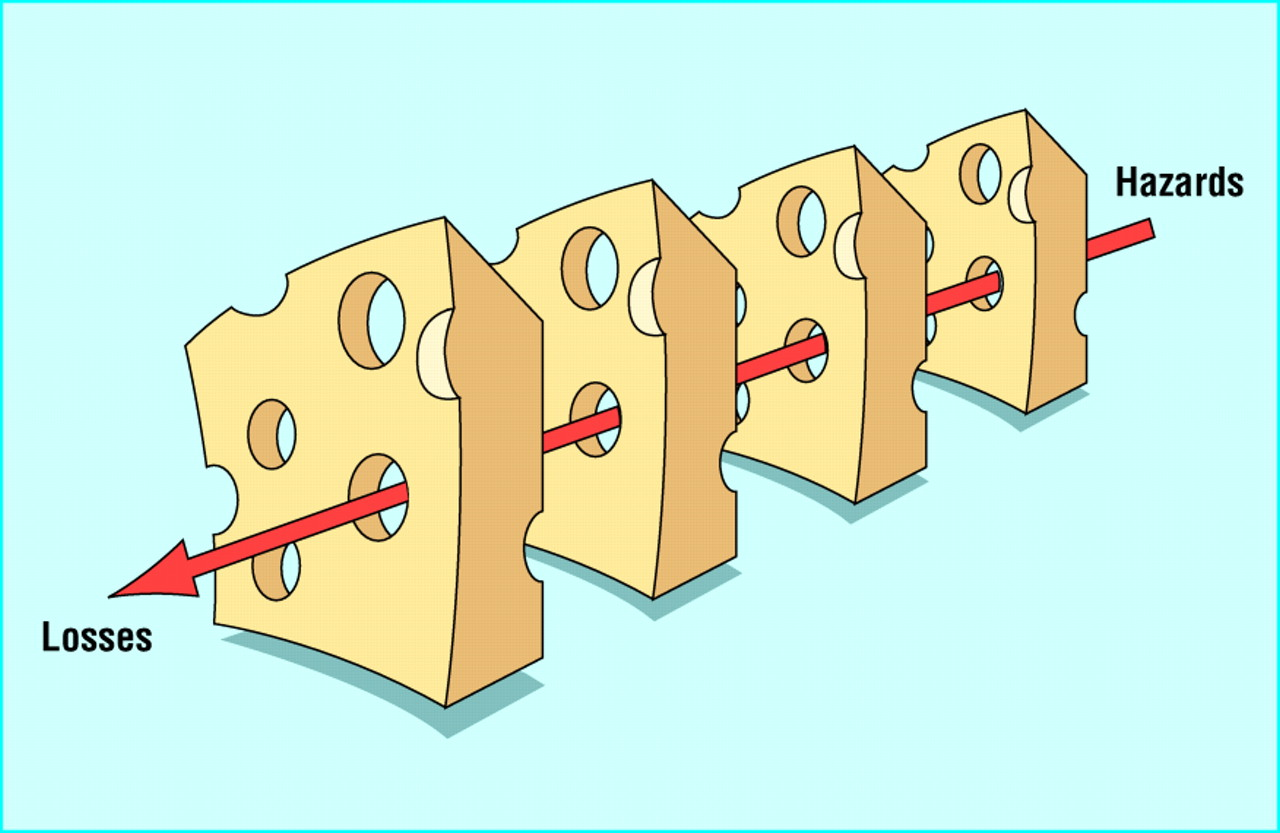
\includegraphics[width=0.8\textwidth]{fig/innledning/sveitserost.jpg}
    \caption{Sveitserostmodellen viser hvordan feil kan skje tross flere lag med sikringstiltak     \citep{HumanErrorModelsManagement}.}
    \label{fig:sveitserost}
\end{figure}

I helsevesenet finnes det mange prosedyrer, protokoller, helsepersonell og utstyr som er ment å forhindre at feil oppstår. Sveitserostmodellen \citep{HumanErrorModelsManagement} vist i figur~\ref{fig:sveitserost} illustrerer hvordan ulike sikkerhetstiltak vanligvis hindrer at en feil fører til pasientskade. Problemet er at alle sikkerhetstiltakene har begrensninger, eller “hull”. En trussel kan dermed passere alle sikkerhetstiltakene i noen tilfeller.  

Når feil skjer i legemiddelhåndteringsprosessen er det pasienten som blir skadelidende. Innsikt i egen legemiddelsituasjon kan gi pasienten bedre forutsetninger for å kontrollere at legemiddelbehandlingen er optimal. 

\subsection*{Dårlig samstemming av legemiddellister}
Bruk av legemidler er et viktig tiltak i helsevesenet, men er ofte lite koordinert og ikke underlagt samlet kontroll. Ulike institusjoner har hver sine lister over hvilke legemidler pasientene står på. Det er påvist at disse listene ofte ikke stemmer overens \citep{vetFast}. 

Internasjonalt blir 25\% av reseptpliktige legemidler pasientene bruker ikke registrert ved innleggelse på sykehus \citep{BCP:BCP204}. Den manglende informasjonen om pasientens legemidler fører til feilbehandlinger og uønskede legemiddelreaksjoner \citep{doi:10.1001/jama.1995.03530010049034}. 

Pasientsikkerhetsprogrammet “I trygge hender” har et mål om å bidra til bedre samstemming av den enkelte pasient sin legemiddelliste. Deres forslag til løsning er at pasienter skal bære med seg en papirutgave av legemiddellisten \citep{Pasientsikkerhetsprosjektet}. Pasientsikkerhetsprogrammet satser på en ikke-elektronisk løsning, i motsetning til andre studier som tilsier at en elektronisk løsning kanskje ville vært bedre \citep{komLegemidler}. En elektronisk oversikt er lettere å holde oppdatert og dele. 

Oversikt over egen legemiddelsituasjon kan føre til at feil som skyldes dårlig samstemming forhindres fordi pasienten har en oppdatert legemiddelliste som kan brukes i kontakt med helsevesenet.

\subsection*{Etterlevelse}
Etterlevelse er et begrep som brukes for å beskrive om legemidler tas som forskrevet. Dårlig etterlevelse er et globalt helseproblem som hindrer pasienter i å få optimal legemiddelbehandling \citep{ConcordanceAdherenceCompliance}. Dårlig etterlevelse medfører dårligere resultat av behandlinger, og økte kostnader for helsevesenet \citep{WHO}. 

Det finnes mange årsaker til dårlig etterlevelse. En årsak er frykt for bivirkninger. I følge apotekforeningen velger 1 av 3 pasienter i Norge å ikke ta legemidlene sine i frykt for bivirkninger \citep{ApotekINorge}. Bedre informasjon om legemidler, som er lettere tilgjengelig, kan bidra til å øke pasientenes etterlevelse \citep{Donovan1992507, doi:10.1056/NEJMra050100}.  

\subsection*{Pasienter som tar flere legemidler}
Antall pasienter med flere kroniske sykdommer\footnote{Kroniske sykdommer: sykdommer med et langtrukkent forløp. Mange kroniske sykdommer er livsvarige, men andre er fullt helbredelige på lang sikt}, og som derfor tar flere legemidler fast, er økende \citep{MultimorbidityPrimaryCare}. Ved bruk av flere legemidler samtidig minker sannsynligheten for god etterlevelse \citep{JOCN:JOCN1477}. 

Pasienter som tar mange legemidler synes ofte det er vanskelig å holde rede på hvorfor de bruker de ulike legemidlene, og når legemidlene skal tas. Antall diagnoser øker med alderen, og eldre pasienter har større vanskeligheter med å oppfatte informasjon og brukerveiledninger \citep{ConcordanceAdherenceCompliance}. 

\section{Forskningsspørsmål} \label{sec:forskningssporsmaal}
Oppgavens bidrag til å nå målet var å gjennomføre et eksperiment som skulle besvare følgende forskningsspørsmål:
\thesisRQ 

Vi utviklet en prototype av et interaktivt system som inneholdt en visuell fremstilling av personlig legemiddelinformasjon. Som vist i figur~\ref{fig:prosess2} var formålet med å utvikle prototypen å bruke den i et eksperiment for å besvare forskningsspørsmålet. I eksperimentet ble prototypen sammenlignet med pakningsvedlegg. Vi valgte å sammenligne med pakningsvedlegg fordi det er en av få eksisterende kilder til legemiddelinformasjon som er rettet mot pasienter. 

\begin{figure}[H]
    \centering
    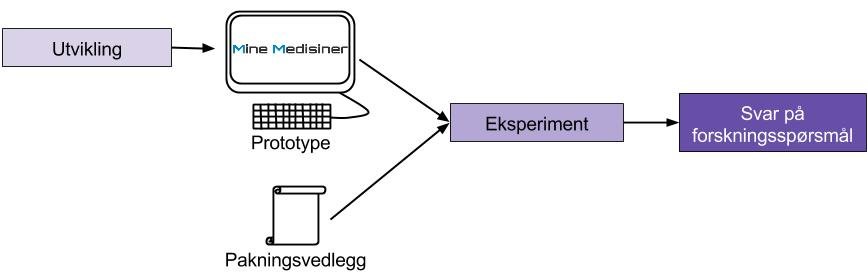
\includegraphics[width=\textwidth]{fig/innledning/prosess.jpg}
    \caption{Arbeidsprosessen mot å besvare forskningsspørsmålet}
    \label{fig:prosess2}
\end{figure}

Basert på forskningsspørsmålet utviklet vi følgende hypoteser:
\begin{enumerate}
 \item Ved å bruke prototypen får pasienter raskere svar på spesifikke spørsmål enn ved å bruke pakningsvedlegg.
 \item Ved å bruke prototypen oppfatter pasienter svaret på spesifikke spørsmål mer korrekt enn ved å bruke pakningsvedlegg.
 \item Ved å bruke pakningsvedlegg tilegner pasienter seg kunnskap utover det de leter etter, i større grad enn ved å bruke prototypen. 
\end{enumerate}


\section{Begrensninger}
I dette delkapittelet presenteres begrensingene til forskningsspørsmålet.

\subsection{Målgruppe} \label{subsec:maalgruppe}
Oppgaven er begrenset til å besvare forskningsspørsmålet for følgende målgruppe:
\begin{quote}Pasienter som tar mer enn ett legemiddel om dagen, og som bruker datamaskin på jevnlig basis.\end{quote}

\subsection{Prototype}
Bruk av et ferdig utviklet system i eksperimentet kunne ført til mer nyttige tilbakemeldinger enn en prototype med mange forenklinger. Programvareutvikling er tidkrevende og var ikke direkte nødvendig for å svare på forskningsspørsmålet. Vi valgte derfor å utvikle en prototype. Prototypen ble utviklet for å fungere for et lite utvalg brukere jf. delkapittel~\ref{sec:personae}. 

\subsection{Personvern}
Vi valgte å avgrense utviklingen av prototypen til å ikke omfatte lagring eller overføring av reelle persondata. Dette ble gjort ved at prototypen kun inneholdt data om de personae som er presentert i oppgaven. Siden prototypen ikke medførte lagring eller overføring av personlige data kunne vi se bort i fra problemstillinger knyttet til personvern. Det er viktig at en ferdig versjon av systemet tar hensyn til problemstillinger knyttet til personvern. Det er en rekke lover, regler og forskrifter som regulerer behandlingen av helseopplysninger, se delkapittel~\ref{sec:sikkerhet}. 

\section{Oppbygging av rapporten}
%\textbf{Kapittel~\ref{chap:innledning}, Innledning:} innholder en gjennomgang av motivasjonen bak oppgaven, samt forskningsspørsmål og begrensninger. Et eksempel på bruk av Mine Medisiner er også presentert. 

\textbf{\autoref{chap:bakgrunn_helsefaglig}, \nameref{chap:bakgrunn_helsefaglig}:} gir utdypning av begrepene interaksjon og bivirkning. 

\textbf{\autoref{chap:bakgrunn}, \nameref{chap:bakgrunn}:} er en gjennomgang av nødvendig bakgrunnsinformasjon om brukergrensesnitt og brukersentrert utvikling. 

\textbf{\autoref{chap:dagensSituasjon}, \nameref{chap:dagensSituasjon}:} presenterer dagens situasjon knyttet til pasienters innsyn i informasjon om egen legemiddelbruk. 

\textbf{\autoref{chap:eksperimentdesign}, \nameref{chap:eksperimentdesign}:} presenterer eksperimentdesignet for oppgaven i form av en overordnet forskningsplan.

\textbf{\autoref{chap:lit}, \nameref{chap:lit}:} er en gjennomgang av relevant litteratur knyttet til problemområdet for oppgaven.

\textbf{\autoref{chap:utviklingsmetoder}, \nameref{chap:utviklingsmetoder}:} beskriver metodene benyttet for å utvikle den digitale prototypen.

\textbf{\autoref{chap:utvikleprototype}, \nameref{chap:utvikleprototype}:} beskriver arbeidet frem mot den digitale prototypen.

\textbf{\autoref{chap:gjennomforing}, \nameref{chap:gjennomforing}:} gir en beskrivelse av forsøket som ble gjennomført for å sammenligne den digitale prototypen og pakningsvedlegg. 

\textbf{\autoref{chap:resultat}, \nameref{chap:resultat}:} presenterer resultatene fra forsøket i form av rådata og tall.
 
\textbf{\autoref{chap:analyse}, \nameref{chap:analyse}:} inneholder påstander som underbygges med resultatene fra forsøket.

\textbf{\autoref{chap:diskusjon}, \nameref{chap:diskusjon}:} inneholder diskusjon av valgene som er tatt, utfordringer som har oppstått underveis og gyldighetene av resultatene.

\textbf{\autoref{chap:konklusjon}, \nameref{chap:konklusjon}:} oppsummerer prosjektet og besvarer forskningsspørsmålet. 

\textbf{\autoref{chap:videreArbeid}, \nameref{chap:videreArbeid}:} inneholder forslag til videre arbeid.
